\documentclass{article}
\usepackage{graphicx, tikz-cd, float, titlepic, booktabs} % Required for inserting images
\usepackage{amsmath, amssymb, amsthm, amsfonts, siunitx, physics, gensymb}
\AtBeginDocument{\RenewCommandCopy\qty\SI}
\usepackage[version=4]{mhchem}
\usepackage[most,many,breakable]{tcolorbox}
\usepackage{xcolor, fancyhdr, varwidth}
\usepackage[Glenn]{fncychap}
%Options: Sonny, Lenny, Glenn, Conny, Rejne, Bjarne, Bjornstrup
\usepackage{hyperref, cleveref}
\usepackage{icomma, enumitem} %comma as decimal and continue enumerate with [resume]
%%%%%%%%%%%%%%%%%%%%%%%%%%%%%%
% SELF MADE COLORS
%%%%%%%%%%%%%%%%%%%%%%%%%%%%%%
\definecolor{myg}{RGB}{56, 140, 70}
\definecolor{myb}{RGB}{45, 111, 177}
\definecolor{myr}{RGB}{199, 68, 64}
\definecolor{mytheorembg}{HTML}{F2F2F9}
\definecolor{mytheoremfr}{HTML}{00007B}
\definecolor{mylenmabg}{HTML}{FFFAF8}
\definecolor{mylenmafr}{HTML}{983b0f}
\definecolor{mypropbg}{HTML}{f2fbfc}
\definecolor{mypropfr}{HTML}{191971}
\definecolor{myexamplebg}{HTML}{F2FBF8}
\definecolor{myexamplefr}{HTML}{88D6D1}
\definecolor{myexampleti}{HTML}{2A7F7F}
\definecolor{mydefinitbg}{HTML}{E5E5FF}
\definecolor{mydefinitfr}{HTML}{3F3FA3}
\definecolor{notesgreen}{RGB}{0,162,0}
\definecolor{myp}{RGB}{197, 92, 212}
\definecolor{mygr}{HTML}{2C3338}
\definecolor{myred}{RGB}{127,0,0}
\definecolor{myyellow}{RGB}{169,121,69}
\definecolor{myexercisebg}{HTML}{F2FBF8}
\definecolor{myexercisefg}{HTML}{88D6D1}
%%%%%%%%%%%%%%%%%%%%%%%%%%%%%%%%%%%%%%%%%%%%%%%%%%%%%%%%%%%%%%%%%%%%%%
% Box environments for theorems and problems
%%%%%%%%%%%%%%%%%%%%%%%%%%%%%%%%%%%%%%%%%%%%%%%%%%%%%%%%%%%%%%%%%%%%%
\setlength{\parindent}{1cm}
%================================
% Question BOX
%================================
\makeatletter
\newtcbtheorem{question}{Opgave}{enhanced,
	breakable,
	colback=white,
	colframe=myb!80!black,
	attach boxed title to top left={yshift*=-\tcboxedtitleheight},
	fonttitle=\bfseries,
	title={#2},
	boxed title size=title,
	boxed title style={%
			sharp corners,
			rounded corners=northwest,
			colback=tcbcolframe,
			boxrule=0pt,
		},
	underlay boxed title={%
			\path[fill=tcbcolframe] (title.south west)--(title.south east)
			to[out=0, in=180] ([xshift=5mm]title.east)--
			(title.center-|frame.east)
			[rounded corners=\kvtcb@arc] |-
			(frame.north) -| cycle;
		},
	#1
}{def}
\makeatother
%================================
% DEFINITION BOX
%================================

\newtcbtheorem[]{Definition}{Definition}{enhanced,
	before skip=2mm,after skip=2mm, colback=red!5,colframe=red!80!black,boxrule=0.5mm,
	attach boxed title to top left={xshift=1cm,yshift*=1mm-\tcboxedtitleheight}, varwidth boxed title*=-3cm,
	boxed title style={frame code={
					\path[fill=tcbcolback]
					([yshift=-1mm,xshift=-1mm]frame.north west)
					arc[start angle=0,end angle=180,radius=1mm]
					([yshift=-1mm,xshift=1mm]frame.north east)
					arc[start angle=180,end angle=0,radius=1mm];
					\path[left color=tcbcolback!60!black,right color=tcbcolback!60!black,
						middle color=tcbcolback!80!black]
					([xshift=-2mm]frame.north west) -- ([xshift=2mm]frame.north east)
					[rounded corners=1mm]-- ([xshift=1mm,yshift=-1mm]frame.north east)
					-- (frame.south east) -- (frame.south west)
					-- ([xshift=-1mm,yshift=-1mm]frame.north west)
					[sharp corners]-- cycle;
				},interior engine=empty,
		},
	fonttitle=\bfseries,
	title={#2},#1}{def}
\newtcbtheorem[]{definition}{Definition}{enhanced,
	before skip=2mm,after skip=2mm, colback=red!5,colframe=red!80!black,boxrule=0.5mm,
	attach boxed title to top left={xshift=1cm,yshift*=1mm-\tcboxedtitleheight}, varwidth boxed title*=-3cm,
	boxed title style={frame code={
					\path[fill=tcbcolback]
					([yshift=-1mm,xshift=-1mm]frame.north west)
					arc[start angle=0,end angle=180,radius=1mm]
					([yshift=-1mm,xshift=1mm]frame.north east)
					arc[start angle=180,end angle=0,radius=1mm];
					\path[left color=tcbcolback!60!black,right color=tcbcolback!60!black,
						middle color=tcbcolback!80!black]
					([xshift=-2mm]frame.north west) -- ([xshift=2mm]frame.north east)
					[rounded corners=1mm]-- ([xshift=1mm,yshift=-1mm]frame.north east)
					-- (frame.south east) -- (frame.south west)
					-- ([xshift=-1mm,yshift=-1mm]frame.north west)
					[sharp corners]-- cycle;
				},interior engine=empty,
		},
	fonttitle=\bfseries,
	title={#2},#1}{def}

\newtcbtheorem{theo}%
    {Theorem}{}{theorem}
\newtcolorbox{prob}[1]{colback=red!5!white,colframe=red!50!black,fonttitle=\bfseries,title={#1}}
%================================
% NOTE BOX
%================================

\usetikzlibrary{arrows,calc,shadows.blur}
\tcbuselibrary{skins}
\newtcolorbox{note}[1][]{%
	enhanced jigsaw,
	colback=gray!20!white,%
	colframe=gray!80!black,
	size=small,
	boxrule=1pt,
	title=\textbf{Note:},
	halign title=flush center,
	coltitle=black,
	breakable,
	drop shadow=black!50!white,
	attach boxed title to top left={xshift=1cm,yshift=-\tcboxedtitleheight/2,yshifttext=-\tcboxedtitleheight/2},
	minipage boxed title=1.5cm,
	boxed title style={%
			colback=white,
			size=fbox,
			boxrule=1pt,
			boxsep=2pt,
			underlay={%
					\coordinate (dotA) at ($(interior.west) + (-0.5pt,0)$);
					\coordinate (dotB) at ($(interior.east) + (0.5pt,0)$);
					\begin{scope}
						\clip (interior.north west) rectangle ([xshift=3ex]interior.east);
						\filldraw [white, blur shadow={shadow opacity=60, shadow yshift=-.75ex}, rounded corners=2pt] (interior.north west) rectangle (interior.south east);
					\end{scope}
					\begin{scope}[gray!80!black]
						\fill (dotA) circle (2pt);
						\fill (dotB) circle (2pt);
					\end{scope}
				},
		},
	#1,
}

%%%%%%%%%%%%%%%%%%%%%%%%%%%%%%%%%%%%%%%%%%%%%%%%%%%%%%%%%%%%%%%%%
% SELF MADE COMMANDS
%%%%%%%%%%%%%%%%%%%%%%%%%%%%%%
\newcommand{\sol}{\setlength{\parindent}{0cm}\textbf{\textit{Løsning:}}\setlength{\parindent}{1cm}}
%%%%%%%%%%%%%%%%%%%%%%%%%%%%%%%%%
\usepackage[tmargin=2cm,rmargin=1in,lmargin=1in,margin=0.85in,bmargin=2cm,footskip=.2in]{geometry}\pagestyle{fancy}
\lhead{Minrui Kevin Zhou 2.b}
\rhead{Matematikaflevering 21}

\title{Aflevering 21\\
{\Large \textbf{2.b mat A}}}
\author{Kevin Zhou}
\date{December 2023}

\begin{document}
\maketitle
\section*{Bedømmelseskriterier:}
\begin{itemize}
    \setlength\itemsep{3cm}
    \Large
    \item  Redegørelse og dokumentation for metode
    \item Figurer, grafer og andre illustrationer
    \item Notation og layout
    \item Formidling og forklaring
\end{itemize}
\pagebreak
\begin{question}{}{}
  Funktionen $f:[0;2\pi[\to \mathbb{R}$ er givet ved
  \[
  f(x)= \sin(x)
  \] 
  \begin{itemize}
    \item[a.] Tegn grafen for $f$.
    \item[b.] Løs ligningen 
    \[
    \sin(x)=\frac{1}{4},\quad 0\leq x < 2\pi
    \] 
  \end{itemize}
\end{question}
\sol \\ 
\textbf{a.} Grafen for $f$ ses i \cref{fig:sin}.
\begin{figure}[H]
\begin{center}
  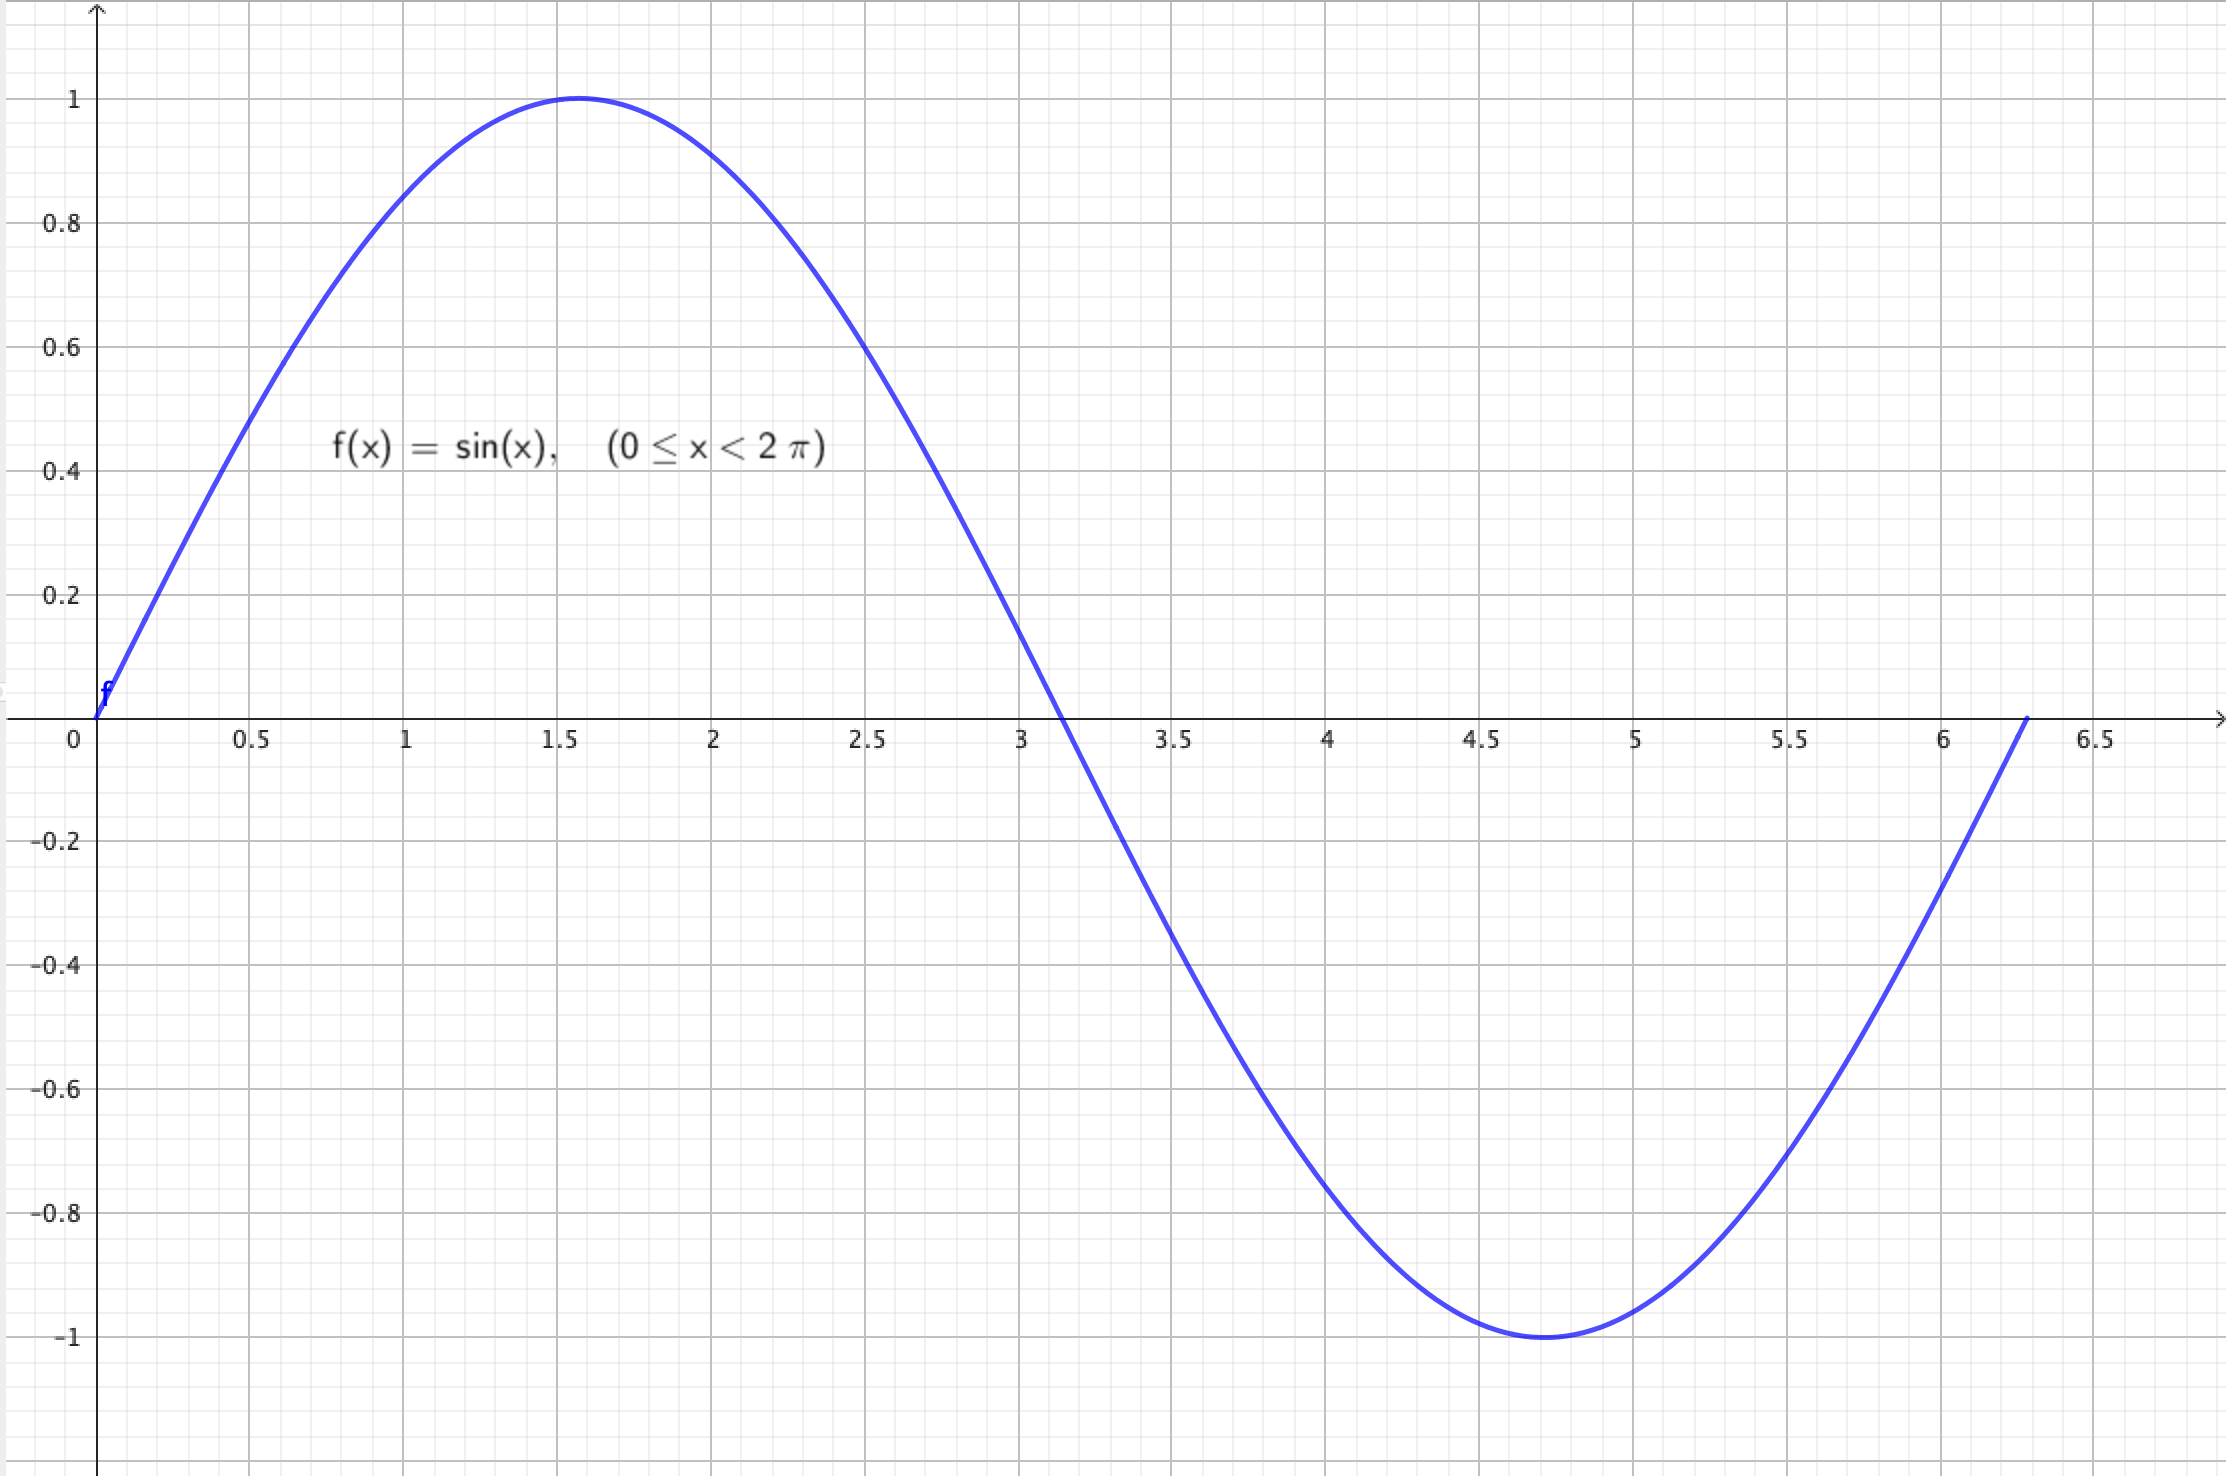
\includegraphics[width=\textwidth]{sin.png}
\end{center}
\caption{Grafen for $f$}
\label{fig:sin}
\end{figure}
\noindent \textbf{b.} Ligningen løses ved hjælp af lommeregneren.
\begin{equation*}
\begin{split}
  \sin(x)=\frac{1}{4} \land 0\leq x < 2\pi &\iff x=\sin^{-1}\left(\frac{1}{4}\right) \lor x=\pi -\sin^{-1}\left(\frac{1}{4}\right) \\
\end{split}
\end{equation*}
\begin{question}{}{}
  Ved en bestemt infektion er antallet af bakterier hos en inficeret person givet ved funktionen 
  \[
  M(t)=3,2 \cdot 10^5 + 7,8\cdot 10^5 \cdot e^{0,154t}
  \] 
hvor $M$ er antallet af bakterier og $t$ er tiden målt i timer. 
\begin{itemize}
  \item[a.] Bestem $M'(18)$, og beskriv hvad dette tal fortæller om udviklingen i antallet af bakterier.
\end{itemize}
\end{question}
\sol \\ 
\textbf{a.} Vi finder den afledede funktion med kædereglen.
\begin{equation*}
\begin{split}
  M'(t)&=0,154 \cdot 7,8 \cdot 10^5 \cdot e^{0,154t}\\ 
  &=1,2012 \cdot 10^5 \cdot e^{0,154t}
\end{split}
\end{equation*}
Vi kan nu tage den aflede funktion for $M$ af $18$.
\begin{equation*}
\begin{split}
  M'(18)&=1,2012 \cdot 10^5 \cdot e^{0,154\cdot 18}\\ 
  &\approx 1,92 \cdot 10^6
\end{split}
\end{equation*}
Dette tal fortæller, at væksthastigheden af bakterierne efter $18$ timer er $1,92 \cdot 10^6$ bakterier per time.

\begin{question}{}{}
  I en model for temperaturen som funktion af tiden i en bestemt by i løbet af et bestemt døgn er temperaturen $f(t)$ målt i grader Celsius til tiden $t$ målt $\mathrm{i}$ antal timer efter midnat givet ved
$$
f(t)=5 \cdot \sin \left(\frac{\pi}{12} t-\frac{5 \pi}{6}\right)+10 ,\;0 \leq t \leq 24
$$
\begin{itemize}
  \item[a.] Tegn grafen for $f$ og bestem temperaturen klokken 7 om morgenen.
  \item[b.] Bestem de tidspunkter på døgnet, hvor temperaturen er 12 grader Celsius.
  \item[c.] Bestem den maksimale temperatur i løbet af døgnet.
  \item[d.] Bestem det tidspunkt på døgnet, hvor temperaturen er maksimal.
  \item[e.] Bestem $f^{\prime}(18)$ og giv en fortolkning af dette tal.
  \item[f.] Bestem det tidspunkt på døgnet, hvor temperaturen stiger mest.
\end{itemize}
\end{question}
\sol \\ 
\textbf{a.} Grafen for $f$ ses i \cref{fig:tid}.
Vi bruger modellen til at finde temperaturen klokken 7.
\begin{equation*}
\begin{split}
  f(7)&= 5 \cdot \sin \left(\frac{\pi}{12} \cdot 7-\frac{5 \pi}{6}\right)+10 \\ 
  &\approx 6,46
\end{split}
\end{equation*}
Altså er temperaturen klokken 7 ifølge modellen $6,46 \;\unit{\celsius}$.
\begin{figure}[H]
\begin{center}
  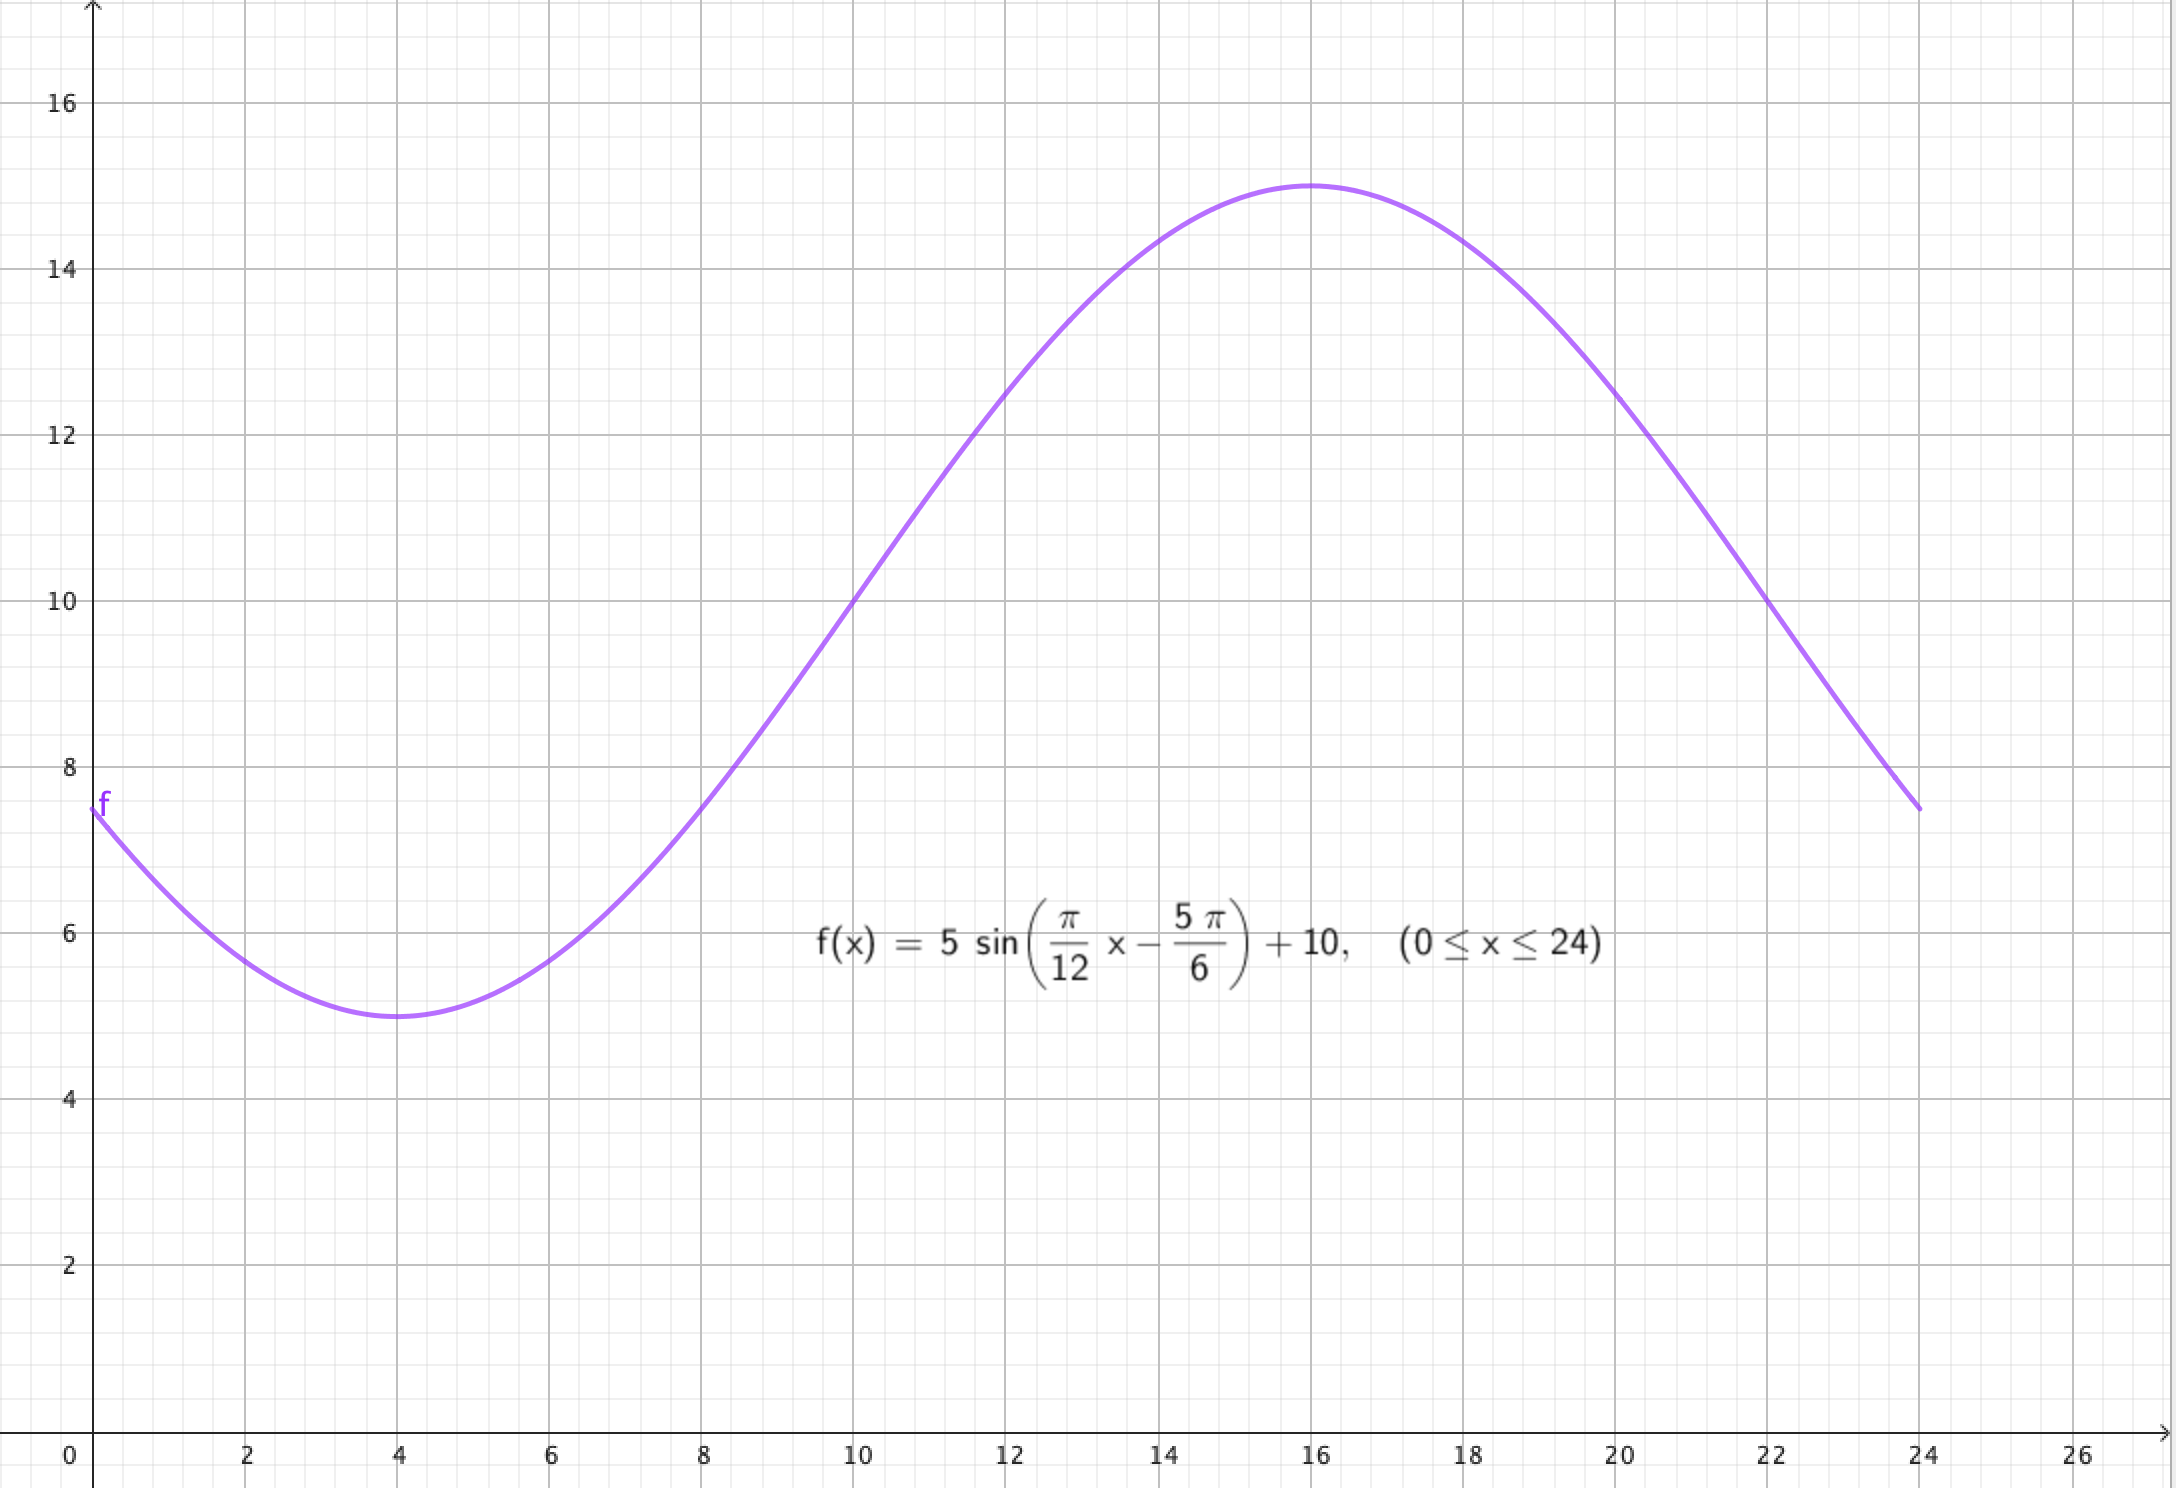
\includegraphics[width=\textwidth]{tid.png}
\end{center}
\caption{Grafen for $f$ tegnet i GeoGebra. Bemærk at variablen hedder $x$ i stedet for $t$ her.}
\label{fig:tid}
\end{figure}
\noindent \textbf{b.}
Vi opstiller en ligning og løser den med hensyn til $x$.
\begin{equation*}
\begin{split}
  f(t)= 12 &\implies 5 \cdot \sin \left(\frac{\pi}{12} t-\frac{5 \pi}{6}\right)+10=12\\ 
  &\iff \sin \left(\frac{\pi}{12} t-\frac{5 \pi}{6}\right)=\frac{2}{5}\\ 
  &\iff \frac{t}{2}\pi - 5\pi = 6 \cdot \sin^{-1}\left(\frac{2}{5}\right)\\ 
  &\iff t=\frac{12\cdot\sin^{-1}\left(\frac{2}{5}\right)}{\pi}+10\\ 
  &\implies t \approx 11,6 \lor t \approx 20,4
\end{split}
\end{equation*}
Altså må temperaturen være $12 \;\unit{\celsius} $ når tiden er enten klokken 11:36 eller klokken 20:24. \\[1ex]
\textbf{c.} Vi finder først den afledede funktion med kædereglen.
\begin{equation*}
\begin{split}
  f'(t)&=5\cdot \cos \left(\frac{\pi}{12} t-\frac{5 \pi}{6}\right) \cdot \frac{\pi}{12} \\ 
  &=- \frac{5}{12} \cdot \pi \cdot \cos \left(\frac{1}{12}\pi \cdot (2+t)\right)
\end{split}
\end{equation*}
Vi sætter dette udtryk lig med 0 og løser for $t$.
\begin{equation*}
\begin{split}
  - \frac{5}{12} \cdot \pi \cdot \cos \left(\frac{1}{12}\pi \cdot (2+t)\right)=0 &\iff \cos \left(\frac{1}{12}\pi \cdot (2+t)\right)=0 \\ 
  &\iff t=\left(\cos^{-1}(0)+\pi n\right) \cdot \frac{12}{\pi} -2, \quad n \in \mathbb{Z}
\end{split}
\end{equation*}
Dog, siden $t \in Dm(f)$, så må der gælde, at 
\[
f'(t)=0 \implies t=4 \lor t=16
\] 
Vi finder nu den dobbeltafledede funktion for $f$ med kædereglen igen. 
\begin{equation*}
\begin{split}
  f''(t)&=\dv{t} \left(- \frac{5}{12} \cdot \pi \cdot \cos \left(\frac{1}{12}\pi \cdot (2+t)\right)\right) \\ 
  &=-\frac{5}{12}\pi \cdot \left(-\sin\left(\frac{1}{12}\pi \cdot (2+t)\right)\right) \cdot \frac{1}{12} \pi \\ 
  &= \frac{5}{144} \pi^2\cdot \sin\left(\frac{1}{12}\pi \cdot (2+t)\right)
\end{split}
\end{equation*}
For at se, om 4 og 16 er maksimumssteder, så tager vi den dobbeltafledede funktion af dem. 
Vi får da, at
\begin{equation*}
\begin{split}
  f''(4) &\approx 0,34 >0 \\ 
  f''(16) &\approx -0,34 < 0
\end{split}
\end{equation*}
Altså må 16 være et maksimumssted. 
Vi regner temperaturen ud, når $t=16$.
\[
f(16)= 5 \cdot \sin \left(\frac{8\pi}{6}-\frac{5\pi}{6}\right)+10 = 15
\] 
Dette må være den maksimale temperatur, da temperaturen ikke er højere i endepunkterne, hvilket nemt kan tjekkes af læseren.
Altså er den maksimale temperatur i løbet af døgnet $15 \;\unit{\celsius} $. \\[1ex]
\textbf{d.} Fra \textbf{c.} får vi, at temperaturen er maksimal, når klokken er 16:00. \\[1ex]
\textbf{e.} Vi har den aflede funktion for $f$ fra \textbf{c.} og tager den af 18.
\begin{equation*}
\begin{split}
  f'(18)&=- \frac{5}{12} \cdot \pi \cdot \cos \left(\frac{1}{12}\pi \cdot (2+18)\right)\\ 
  &=- \frac{5}{12} \cdot \pi \cdot \frac{1}{2} \\
  &=-\frac{5}{24}\pi
\end{split}
\end{equation*}
Dette tal fortæller da, at temperaturen til tidspunktet $t=18$ aftager med $\frac{5}{24}\pi \;\unit{\celsius} $ per time. \\[1ex]
\textbf{f.}  
Vi løser da ligningen $f''(t)=0$ med hensyn til $t$.
\begin{equation*}
\begin{split}
  \frac{5}{144} \pi^2\cdot \sin\left(\frac{1}{12}\pi \cdot (2+t)\right)=0 &\iff \sin\left(\frac{1}{12}\pi \cdot (2+t)\right)=0 \\ 
  &\iff t=\left(\sin^{-1}(0)+\pi n\right) \cdot \frac{12}{\pi}-2, \quad n \in \mathbb{Z}
\end{split}
\end{equation*}
Siden $t \in Dm(f)$, så må der gælde, at
\[
f''(t)=0 \implies t=10 \lor t=22
\] 
Vi hævder, at disse er ekstremumssteder, hvilket nemt kan tjekkes af læseren vha. den triple-afledede funktion for $f$.
Altså er stiger temperaturen mest klokken 10:00 og 22:00.

\begin{question}{B}{}
 Figuren er et lodret snit $ABCD$ gennem en kanal, hvis tværsnit har form som et trapez.
  Arealet af kanalens tværsnit er en funktion $T$ af vinklen $v$, hvor $v$ måles i radianer og $0<v\leq \frac{\pi}{2}$. 
  \begin{itemize}
    \item[a.] Gør rede for, at
    \[
    T(v)=8 \sin v + 4 \sin v \cos v
    \] 
    og bestem $v$, så arealet af tværsnittet bliver størst muligt.
  \end{itemize}
\end{question}
\begin{figure}[H]
\begin{center}
  \includegraphics[width=0.7\textwidth]{tværsnit.png}
\end{center}
\caption{Tværsnit af kanalen}
\label{fig:kanal}
\end{figure}
\sol \\ 
\textbf{a.} Lad $h$ betegne den lodrette side af de to retvinklede trekanter, og lad $x$ betegne længden af den vandrette side. 
Så må der da gælde, at 
\begin{equation*}
\begin{split}
  h&=2\cdot \sin v \\
  x&=2\cdot \cos v
\end{split}
\end{equation*}
Arealet af trapezen må være arealet af den store rektangel med de to treanters arealer trukket fra:
\begin{equation*}
\begin{split}
  T(v)&=(4+2x)\cdot h - hx \\
  &=4h + hx \\ 
  &=8 \sin v + 4 \sin v \cos v
\end{split}
\end{equation*}
hvilket var, hvad vi skulle vise.

Vi finder nu den aflede funktion for $T$ med hensyn til $v$ med produktreglen og sætter dette udtryk lig med 0 og løser for $v$.
\begin{equation*}
\begin{split}
  T'(v)&=8 \cos v + 4 \left(\cos^2 v - \sin^2 v\right) =0 \\ 
  &\implies 2 \cos v + 2 \cos^2 v - 1 =0 \\ 
  &\iff \frac{1}{4} + \cos v + \cos^2 v = \frac{3}{4} \\ 
  &\iff \cos v + \frac{1}{2} = \pm \frac{\sqrt{3} }{2} \\ 
  &\iff v=\cos^{-1} \left(\pm \frac{\sqrt{3} -1}{2}\right) +2\pi n,\quad n \in \mathbb{Z}
\end{split}
\end{equation*}
Dog, siden $0<v\leq \frac{\pi}{2}$, så må det gælde, at
\[
T'(v)=0 \implies v =\cos^{-1}\left(- \frac{\sqrt{3} -1}{2}\right) \lor v =\cos^{-1}\left( \frac{\sqrt{3} -1}{2}\right)
\]
Vi finder nu den dobbeltafledede funktion for $T$ med hensyn til $v$ med produktreglen. 
\begin{equation*}
\begin{split}
  T''(v)&= \dv{v} \left(2 \cos v + 2 \cos^{2} v - 1\right) \\ 
  &= -2\sin v - 4 \cos v\sin v \\ 
  &= -2\sin v \left(2\cos v + 1\right) 
\end{split}
\end{equation*}
Vi får ved indsættelse i denne funktion, at
\begin{equation*}
\begin{split}
  T''\left(\cos^{-1}\left(- \frac{\sqrt{3} -1}{2}\right)\right) &<0 \\ 
  T''\left( \cos^{-1}\left( \frac{\sqrt{3} -1}{2}\right)\right) &<0
\end{split}
\end{equation*}
Vi finder arealet, ved disse to vinkler.
\begin{equation*}
\begin{split}
  T''\left(\cos^{-1}\left(- \frac{\sqrt{3} -1}{2}\right)\right) &\approx 6,08 \\ 
  T''\left( \cos^{-1}\left( \frac{\sqrt{3} -1}{2}\right)\right)  &\approx 8,81
\end{split}
\end{equation*}
Altså må arealet af tværsnittet være størst når 
\[
v=\cos^{-1}\left(- \frac{\sqrt{3} -1}{2}\right)
\] 
\end{document}
